%%%%%%%%%%%%%%%%%%%%%%%%%%%%%%%%%%%%%%%%%%%%%%%%%%%%%%%%%%%%%%%%%%%%%%%%%%%%%%%%
% reconstruction.tex:
%%%%%%%%%%%%%%%%%%%%%%%%%%%%%%%%%%%%%%%%%%%%%%%%%%%%%%%%%%%%%%%%%%%%%%%%%%%%%%%%
\chapter{Event Reconstruction and Selection}
\label{sec:reco_chapter}
%%%%%%%%%%%%%%%%%%%%%%%%%%%%%%%%%%%%%%%%%%%%%%%%%%%%%%%%%%%%%%%%%%%%%%%%%%%%%%%%

Electrons, muons and jets expected from \WR and \nul decays traverse multiple CMS sub-detectors, as shown in 
Figure \ref{fig:particleTrajectories}.  Their trajectories and energies were measured from charged particle tracks 
reconstructed by the silicon tracker and muon detectors, and energy deposits reconstructed by the calorimeters.  The 
high energy of expected leptons and jets motivated the use of specific lepton and jet reconstruction algorithms 
described here.  These algorithms combine measurements from multiple CMS sub-detectors to measure the trajectory 
and energy of each particle with optimal resolution.  For charged particles, initial energy and trajectory 
measurements are made using tracks reconstructed from signals measured in the silicon tracker.

\begin{figure}[h]
	\centering
	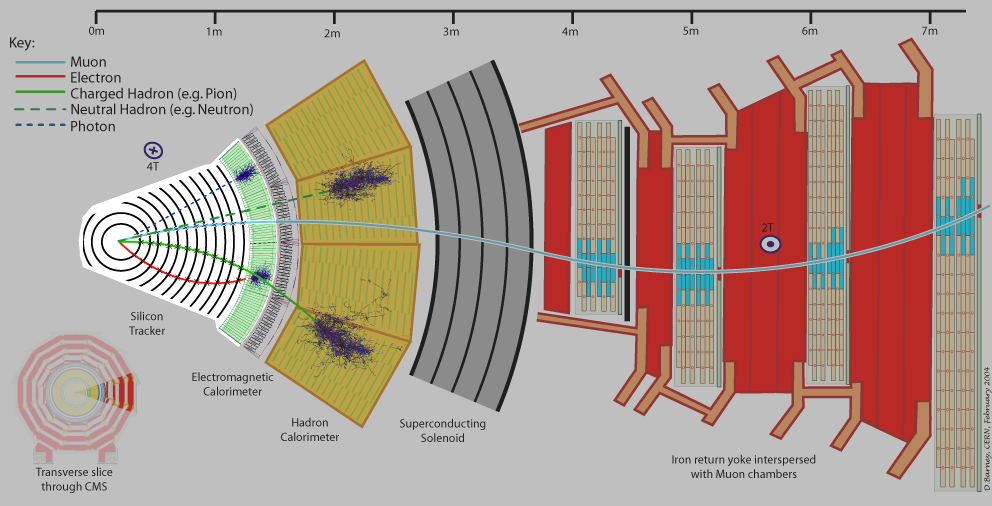
\includegraphics[width=0.75\textwidth]{figures/flowOfParticlesThroughCMS.png}
	\caption{Typical trajectories of particles travelling through CMS, from CERN.}
	\label{fig:particleTrajectories}
\end{figure}


\section{Track Reconstruction}
\label{sec:trkReco}
Charged particles are reconstructed as helical tracks from signals measured in the silicon tracker.  An interative algorithm 
starts by reconstructing tracks from signals in the inner pixel tracker characterized by the highest energies or smallest 
distances from the IP, and progressively includes signals measured in outer pixel tracker and silicon strip tracker layers.  
Signals in successive layers are linked into continuous tracks using a Kalman filter that requires each signal to have 
$\chi^{2} <$ 30 \cite{trackerPerformanceInCollisions}.  Each time a new signal is added to a track, an analytic function 
extrapolates the track trajectory to the next layer assuming energy is lost only through ionization in the silicon.  Hits in 
the next layer are searched for in the region identified by the analytic function extrapolation, and this procedure repeats 
until signals are included from the outermost silicon strip tracker layer.  Then, the signals linked into tracks are removed 
from the list of track candidates, and the algorithm restarts using signals measured in the inner pixel tracker characterized 
by lower energies or larger distances from the IP.  Using this algorithm, isolated muons with $\pt > 0.9$ $\GeV$ and $|\eta| < 2.4$ 
were reconstructed as tracks with essentially 100\% efficiency \cite{trackerPerformanceInCollisions}.  After reconstructing 
all tracks in an event, each point where two or more tracks originate is identified as an interaction vertex, and its position 
is measured relative to the IP.  The positions of vertices that have muon tracks with $|\eta| < 1.4$ and $\pt = 100$ $\GeV$ 
were measured with 10 and 30 $\mu$m resolutions in the transverse (r-$\phi$) and longitudinal ($z$) directions.

The track reconstruction algorithm described previously is used to reconstruct muon and charged hadron tracks, but a second 
algorithm is used to reconstruct electron tracks.  The silicon tracker contains, depending on $\eta$, 1 to 2 radiation 
lengths of material that causes electrons to shower.  As a result, $\sim$35\% of electrons that traverse the tracker lose more 
than 70\% of their initial energies through bremsstrahlung \cite{trackerPerformanceInCollisions}, which cannot be measured by 
the tracker.  The electron track reconstruction algorithm uses the same iterative track reconstruction procedure described 
previously, but extrapolates each track's trajectory to the next silicon layer assuming the energy lost through bremsstrahlung 
is described by a sum of Gaussians.  In addition, the Kalman filter used to link signals in successive layers requires that new 
signals have $\chi^{2} <$ 2000.  The electron track algorithm reconstructed electrons with $\pt > 20$ $\GeV$ and $|\eta| < 2.5$ 
as tracks with 97\% or better efficiency \cite{gsfPerformanceInCollisions}.


\section{Energy Reconstruction}
\label{sec:enrgReco}
The energies of photons, electrons, and hadrons produced by pp interactions are measured in groups of ECAL crystals.  Photons, 
electrons, and hadrons impinging on the ECAL generate signals in the ECAL crystals that are converted into uncalibrated energies.  Groups, 
or superclusters (SCs), of crystals are built from the most energetic crystals with $\Et \gtrsim 0.2$ $\GeV$ and their nearest 
neighbors, and are at least 3 crystals wide in $\eta$.  The upstream tracker material causes $\sim$35\% of electrons and 
photons, and up to 25\% of hadrons \cite{trackerPerformanceInCollisions} to shower in the tracker, and radiate energy by emitting 
photons and other particles.  The energy is typically radiated along the particle's $\eta$ trajectory, but spread over several ECAL 
crystals in $\phi$.  To capture this energy, each SC is at least 5 crystals wide in $\phi$, and can be much larger, as in 
Figure \ref{fig:eleTrackAndSC}.  Once a SC is built, the energy of each crystal in the SC is multiplied by a laser 
transparency correction, and relative and absolute energy calibration corrections.  The sum of the calibrated crystal energies 
is the SC energy, and the energy weighted average $(\eta,\phi)$ position is the SC position.  Using only ECAL SCs, the $(\eta,\phi)$ 
positions of electrons in the barrel (endcap) were measured with a $\phi$ resolution of 0.17$^{\circ}$ (0.29$^{\circ}$), and an 
$\eta$ resolution of 0.001 (0.002) units.

The energies of hadrons that traverse the ECAL are measured in groups of HCAL towers.  Hadrons impinging on the HCAL generate signals 
in the HCAL towers that are converted into uncalibrated energies.  The highest energy towers with $\Et \gtrsim 1$ $\GeV$ are used to 
seed clusters, which extend to all neighboring towers with $\Et > 0.8$ $\GeV$ \cite{pflowEventReco}.  If one tower is grouped into 
multiple clusters, the tower's contribution to each cluster is weighted by its distance from each cluster's seed.  After clusters are 
built, each tower's energy is multiplied by a laser transparency correction, and relative and absolute energy calibration corrections.  
The sum of the calibrated tower energies is the cluster energy, and the energy weighted average $(\eta,\phi)$ position is the cluster 
position.  Hadron energies are measured as a combination of calibrated HCAL cluster energies, and energies of overlapping ECAL SCs.  
Using the combined ECAL-HCAL system, hadrons with $\Et = 100$ $\GeV$ were measured with a $\sim$10\% $\Et$ resolution \cite{pflowEventReco}.


\section{Muon Reconstruction and Selection}
\label{sec:muReco}

\subsection{Reconstruction}
Muons are first reconstructed as tracks from signals measured in individual muon chambers.  In each DT chamber, the start and end points of 
track segments are identified first as pairs of signals measured in the same plane (r-$\phi$ or r-z) but in different layers.  Then straight 
lines are drawn between the signal pairs, and a signal pair is ignored if its line is not compatible with a track that extrapolates from 
the chamber to the IP.  The remaining signals that are consistent with any of these straight lines are built into track segments that are 
measured in at least 3 layers.  In each plane the track segment with signals in the largest number of layers, at least 3, and the lowest 
$\chi^{2}/nDOF$, less than 20, is used to build a 3D track.  In the event where more than one track segment is reconstructed 
in one plane of a DT chamber, all combinations of r-$\phi$ and r-z track segments are considered when reconstructing a 3D track.  In 
practice, more than one 3D track is reconstructed in a DT chamber in less than 1\% of events \cite{cmsTdrPhysPerformance}.  The same 
track segment reconstruction algorithm is used in each 6 layer, single plane CSC.  There the final track segment must have signals 
in at least 4 layers.  In the barrel-endcap transition region, $1.3 < |\eta| < 1.6$, where the DT chambers stop and the CSCs begin, RPCs 
are used to improve the muon reconstruction efficiency and the precision of arrival time measurements.  Each RPC contains two parallel 
plates divided into many thin strips, and strips that measure a signal are grouped into clusters.  Each reconstructed cluster represents 
a hit whose position is the 'center of gravity' of all the strips in the cluster.

Tracks reconstructed in individual chambers are used to reconstruct muon trajectories through the magnetic field and all muon chambers.  
A Kalman filter algorithm starts with tracks in the chambers closest to the IP, and predicts the track positions in chambers in the next 
radial station with the effects of an inhomogeneous magnetic field and material losses taken into account \cite{muonRecoFirstCollisions}.  
Track segments in outer chambers are added to existing tracks subject to a $\chi^{2}$ requirement, and existing tracks are propagated to 
the next radial station even if no matching track segment is found in the current station.  Once the outermost station is included, a 
reverse Kalman filter is applied to reconstructed tracks from the outermost station working to the innermost station.  The reverse Kalman 
filter finalizes the track parameters, then these tracks are compared to silicon tracker tracks to identify global muons.

Global muons are identified using tracks reconstructed in the silicon tracker and muon detectors.  Tracks from the muon detectors are 
extrapolated back to the outermost silicon tracker layer, and their positions are compared.  In the local coordinate plane of the 
silicon strip layer, each silicon tracker track that matches a muon detector track within 3 cm is identified as a global muon.  If an 
extrapolated muon detector track has multiple silicon tracker track candidates within 3 cm, the closest match is used to make a global 
muon.  The matched silicon tracker track determines the $(\eta,\phi)$ trajectory of each global muon.

The momentum of each global muon is determined by sampling four different global muon reconstruction algorithms, and selecting the  
highest quality result.  Each algorithm fits a continuous track \cite{cmsMuonRecoRunTwo} to a unique combination of silicon tracker 
and muon detector signals to estimate a muon's trajectory through CMS, depicted in Figure \ref{fig:particleTrajectories}.  The 
quality of each continuous track is identified by a fit uncertainty $\chi^{2}/nDOF$ and momentum uncertainty $\sigma(\pt)/\pt$; and 
the track with the lowest $\chi^{2}/nDOF$ and momentum uncertainty $\sigma(\pt)/\pt < 0.3$ determines the global muon's momentum.  
For muons with $\pt \lesssim 100$ $\GeV$ the highest quality result is obtained using only silicon tracker measurements.  Muons with 
$|\eta| < 1.4$ and $\pt = 100$ $\GeV$ were measured with a $\pt$ resolution of $\sim$2.8\% \cite{trackerPerformanceInCollisions}.  
However, as a muon's $\pt$ increases above 100 $\GeV$ the silicon tracker $\pt$ resolution degrades faster that that of the muon 
detectors.  A significant fraction of $\WR \rightarrow \mu\mu jj$ events are expected to produce at least one muon with $\pt > 200$ $\GeV$ 
(Table \ref{tab:wrHighPtMuons}), and in this high $\pt$ region the highest quality momentum measurement is made by combining silicon 
tracker and muon detector measurements.  Muons with $|\eta| < 0.9$ and $200 < \pt < 400$ $\GeV$ were measured with a $\pt$ resolution 
of 3.2\%, and higher $\pt$ muons were measured with a resolution better than 6\% \cite{cmsMuonRecoRunTwo}.

\begin{table}[h]
	\caption{Fraction of expected $\WR \rightarrow \mu\mu jj$ events that had at least one muon with $\pt > 200$ $\GeV$. 
	($\mnul = \frac{1}{2}\mWR$)}
	\label{tab:wrHighPtMuons}
	\centering
	\begin{tabular}{c|c}
		\mWR ($\TeV$) & Fraction of events with at least one high-$\pt$ muon (\%) \\  \hline
		1.0 &  80.  \\
		2.0 &  95.  \\ 
		3.0 &  98.  \\ \hline
	\end{tabular}
\end{table}

Global muons reconstructed in simulated events are known to have different energies than muons reconstructed in data.  Energy 
corrections for simulated muons are derived using $Z \rightarrow \mu\mu$ events found in simulations and data.  The di-muon mass 
($M_{\mu\mu}$) distribution in $Z \rightarrow \mu\mu$ events is compared between data and simulations, and the energies of muons 
in simulated events are corrected so that the two $M_{\mu\mu}$ distributions match.

\subsection{Online Selection}
During collisions events with muons were selected using a single muon Level-1 trigger.  The trigger required one reconstructed 
track segment with $\pt > 16$ $\GeV$ that spanned one DT or CSC chamber in at least 2 stations, and the track segment in each chamber 
was built from signals in at least 4 layers.  Then, events were required to pass the following single muon HLT selection criteria:

\begin{itemize}
	\item A track reconstructed in the silicon tracker with $\pt > 50$ $\GeV$ and $|\eta| < 2.4$ was geometrically matched to 
		the muon detector track segment that passed the L1 trigger.
	\item In the plane perpendicular to the beam axis, the distance between the silicon tracker track origin and its 
		reconstructed vertex was $< 1$ mm.
\end{itemize}

\subsection{Offline Identification Selection}
In events selected by the single muon trigger, muons were reconstructed offline from muon detector and silicon tracker tracks using 
algorithms described previously.  After reconstruction, the following identification criteria were applied to select promptly produced, 
isolated muons that were reconstructed in multiple muon stations:

\begin{itemize}
	\item The muon track reconstructed in the silicon tracker:
	\begin{itemize}
		\item Was reconstructed from a signal in at least 1 silicon pixel detector layer, and signals in at least 
			5 layers in the entire tracker.
		\item Within a cone of radius $\Delta R = 0.3$ centered on the track, the $\sum \pt$ of all other 
			reconstructed tracks was low compared to the muon $\pt$, $\frac{\sum \pt}{\mu \pt} < 0.1$.
	\end{itemize}
	\item The muon was reconstructed in the muon detectors as a track segment that spanned one chamber in at least 
		2 muon stations.  Track segments in each DT chamber were required to have signals in all 4 r-$z$ layers, and 
		at least 7 of 8 r-$\phi$ layers.  Track segments in each CSC were required to have signals in all 6 layers.
	\item The origin of the muon's silicon tracker track was within 2 mm of the muon's reconstructed vertex 
		position along the $z$ axis.
\end{itemize}


\section{Electron Reconstruction and Selection}
\label{sec:eleReco}

\subsection{Reconstruction}
Electrons are the only particles from \WR decays expected to lose more than a few percent of their initial energy through 
bremsstrahlung in the tracker.  A dedicated electron track reconstruction algorithm is used to reconstruct tracks from electrons, 
even those that experience large energy losses, with high efficiency, but the tracker cannot measure the magnitude of bremsstrahlung 
energy losses.  However, the energies of electrons and their bremsstrahlung photons are measured by the ECAL.  Therefore, the ECAL 
is used to measure the $\Et$ and $(\eta,\phi)$ trajectory of each electron.

Electrons are identified using reconstructed tracks and ECAL SCs.  Reconstructed tracks are extrapolated from the outermost 
silicon strip layer to the front face of the ECAL, and their positions are compared to ECAL SCs.  Each electron is identified 
as one or more tracks that match the SC $(\eta,\phi)$ position within 1.1$^{\circ}$, about 1 crystal wide, in $\phi$, and 
within 0.004 units, less than $\frac{1}{2}$ a crystal wide, in $\eta$.  In addition, the ECAL SC $\Et$ and the matched 
track $\pt$ must agree within the uncertainty on the track $\pt$.  Using the SC energy, electrons with $\Et \approx 45$ 
$\GeV$ and $|\eta| < 0.8$ were measured with an $\Et$ resolution better than 2\%, and a resolution between 2\% and 5\% 
at higher $|\eta|$ \cite{ecalPerformanceInCollisions}.

\begin{figure}[h]
	\centering
	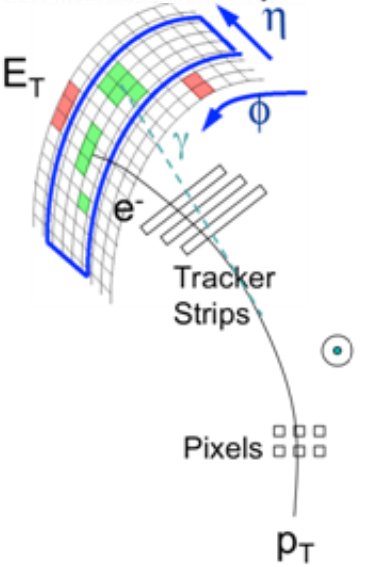
\includegraphics[width=0.75\textwidth]{figures/electronTrackAndSupercluster.png}
	\caption{The trajectory of a typical electron through the tracker and the ECAL.}
	\label{fig:eleTrackAndSC}
\end{figure}

Electrons reconstructed in simulated events are known to have different energies than electrons reconstructed in data.  Energy 
corrections for simulated electrons are derived using $Z \rightarrow ee$ events found in simulations and data.  The di-electron mass 
($M_{ee}$) distribution in $Z \rightarrow ee$ events is compared between data and simulations, and the energies of electrons 
in simulated events are corrected so that the two $M_{ee}$ distributions match.

\subsection{Online Selection}
During collisions events with electrons were selected using single and double-electron Level-1 triggers.  These triggers required 
either one 5 $\times$ 5 ECAL crystal cluster reconstructed with $\Et > 40$ $\GeV$, or two 5 $\times$ 5 ECAL clusters: one with 
$\Et > 22$ $\GeV$, the other with $\Et > 10$ $\GeV$.  Then, events were required to pass the following double-electron HLT selection 
criteria:

\begin{itemize}
	\item Two 5 $\times$ 5 ECAL crystal clusters separated by $\Delta R > 0.1$ were reconstructed with $\Et > 33$ $\GeV$.
	\item For each ECAL cluster:
	\begin{itemize}
		\item The ratio of energy (H) in the HCAL tower behind the cluster to the cluster energy (E) was $\frac{H}{E} < 0.15$ 
			in the barrel, and $\frac{H}{E} < 0.1$ in the endcap.
		\item Ninety percent of the cluster energy was measured in an area that was two crystals wide in $\eta$.
		\item If the cluster was in the barrel, a reconstructed track with signals in at least two pixel tracker layers 
			extrapolated close to the cluster position.  The track extrapolated from the pixel tracker to within $2.3$ cm 
			of the ECAL cluster $z$ position, and to within 1 ECAL crystal area of the cluster $(\eta,\phi)$ position.
	\end{itemize}
\end{itemize}

\subsection{Offline Identification Selection}
In events selected by the double-electron trigger, electrons were reconstructed offline from ECAL SCs and tracks using algorithms 
described previously.  After reconstruction, the following identification criteria were applied to select promptly produced 
electrons that did not lose significant energy in the tracker, and were not reconstructed near a jet:

\begin{itemize}
	\item Electrons reconstructed with $1.44 < |\eta| < 1.57$ were ignored.
	\item For barrel electrons, at least 94\% of the SC energy was measured in an $\eta$ region that was 2 crystals 
		wide.
	\item The ratio of energy (H) in the HCAL tower behind the SC to the SC energy ($E_{SC}$) was $\frac{H}{E_{SC}}< 0.05 + \frac{1}{E_{SC}}$ 
		in the barrel, and $\frac{H}{E_{SC}}< 0.05 + \frac{5}{E_{SC}}$ in the endcap.
	\item In a $\Delta R =$ 0.3 radius cone centered on the electron's $(\eta, \phi)$ trajectory:
	\begin{itemize}
		\item The $\sum \pt$ of all tracks excluding the electron's track was low, $\sum \pt < 5$ $\GeV$.
		\item The total calorimeter energy $E_{ECAL + HCAL}$ in the cone not associated with the electron was low, 
			$E_{ECAL + HCAL} < 2 + 0.03\alpha + 0.28\rho$.  $\rho$ was the neutral particle energy per unit $\eta,\phi$ area, 
			$\alpha$ in the barrel was the electron $\Et$, and $\alpha$ in the endcap was the electron $\Et - 50$.
	\end{itemize}
	\item The electron track extrapolated from the outermost silicon tracker measurement to within $\sim$3 crystal 
		widths in $\phi$ of the SC seed crystal position.
	\item The electron track was built from signals in every silicon pixel and inner strip detector layers, or all but 1 layer.
	\item The electron track's origin was separated from its vertex by a small distance $\Delta_{xy}$ in the $x-y$ 
		plane: $\Delta_{xy} < 0.2$ mm in the tracker barrel, and $\Delta_{xy} < 0.5$ mm in the tracker endcap.
\end{itemize}


\section{Jet Reconstruction and Selection}
\label{sec:jetReco}

\subsection{Reconstruction}
Quarks and gluons emitted from pp interactions produced jets of photons, hadrons and leptons.  On average, 85\% of a jet's 
energy is carried by charged particles and photons \cite{pflowJetRecoInCollisions}, so these particles are prioritized during 
jet reconstruction.  The particle flow jet reconstruction algorithm \cite{pflowEventReco} identifies $(\eta,\phi)$ regions 
with one or more silicon tracker or muon detector tracks, one or more HCAL energy clusters, and any number of ECAL 
SCs.  In these regions, algorithms described previously are used to reconstruct muons first, followed by electrons.  Tracks and 
energy deposits identified as leptons are removed from the list of particle candidates.  The remaining tracks and energy clusters 
are used to identify charged hadrons, photons, and neutral hadrons.  Each charged hadron is identified as a track matched to an HCAL 
cluster and possibly an ECAL SC, and the charged hadron's $\pt$ and $(\eta,\phi)$ trajectory are determined by the track.  The track 
$\pt$ must agree with the total calorimeter $\Et$ within the calorimeter $\Et$ uncertainty.  Each photon is identified as an ECAL SC 
that are not geometrically matched to a track or HCAL cluster whose $\pt$ or $\Et$ agrees with the SC $\Et$ within the ECAL $\Et$ 
uncertainty.  Finally, each neutral hadron is identified as an HCAL cluster and any overlapping ECAL SC that are not geometrically 
matched to a track whose $\pt$ agrees with the calorimeter $\Et$ within the calorimeter $\Et$ uncertainty.  After all tracks and 
energy clusters in a region are identified as specific particles, a jet, represented by the cone in Figure \ref{fig:jetClustering}, 
is clustered from those particles.

Due to the high instantaneous collision luminosity, each pp bunch crossing delivered by the LHC produces multiple pp interactions, 
or pileup (PU) interactions, that make jet clustering more challenging.  In every unit of $\eta$, each PU interaction adds 
$\sim$11 charged particle tracks with $\pt \approx 0.5$ $\GeV$ to the event \cite{chgdHdrMultInData}.  These tracks are primarily 
charged hadrons, so before jets are clustered the charged hadrons associated with PU interaction vertices are removed from 
all jet clustering regions.  Jets are then clustered from reconstructed particles using the anti-$k_{T}$ algorithm \cite{antikt} 
with a cone size of $\Delta R = 0.4$.  In each region the anti-$k_{T}$ algorithm starts with the highest $\pt$ hadron and adds 
other particles to the jet cone based on their $\pt$ and distance from the jet axis.  A cone size of $\Delta R = 0.4$ is used to 
cluster lower area jets that are less sensitive to PU contamination, but does not prohibit jets from being clustered with radius 
$\Delta R > 0.4$.  Once jets are clustered a second technique is used to reduce the contribution of neutral particles produced in PU interactions 
to jet energies.  This technique uses the $k_{T}$ algorithm \cite{ktAlgoOne,ktAlgoTwo,ktAlgoThree} with cone size $\Delta R = 0.3$ 
to cluster jets from all particles reconstructed in the event, including jets that only contain neutral particles.  
Each $k_{T}$ jet's $\pt$ is divided by the jet's area ($\pt_{j} / A_{j}$), and the median value $\rho$ is used as the average neutral 
particle energy density in the event \cite{pileup1,pileup2}.  Using the hybrid jet area subtraction technique described in 
\cite{pflowJetRecoInCollisions}, the photon and neutral hadron energies in each anti-$k_{T}$ jet are reduced based on $\rho$, and each 
jet's area and $\eta$.  After all subtractions, jet energies are calibrated to correct for known variations in the detector response to jets 
as functions of $\eta$ and $\pt$.  By combining measurements from the silicon tracker, calorimeters, and muon detectors, particle 
flow jets with $\pt > 40$ $\GeV$ and $|\eta| < 2.4$ were measured with a $\pt$ resolution better than 13\% \cite{jetResolutionInCollisions}.

\begin{figure}[h]
	\centering
	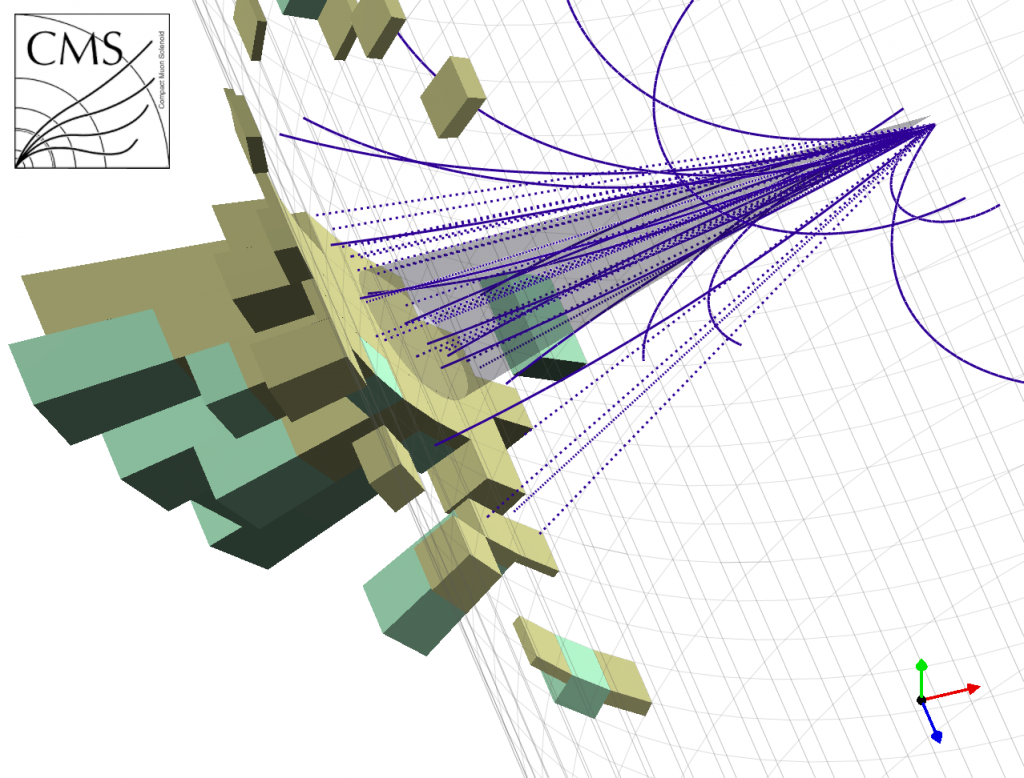
\includegraphics[width=0.75\textwidth]{figures/jetClusteringInCMS.png}
	\caption{A cone of reconstructed particles clustered into a jet, with the reconstructed vertex on the right.  
	From the CMS Experiment.}
	\label{fig:jetClustering}
\end{figure}

Jets reconstructed in simulated events are known to have different energies than jets reconstructed in data.  Energy corrections for 
simulated jets are derived using dijet, $Z$+jet, and $\gamma$+jet events found in simulations and data 
\cite{jetpaper}.  The di-jet mass and leading jet $\pt$ distributions in these events are compared between data and simulations, and 
the energies of jets in simulated events are corrected so that the jet distributions match in data and simulations.

\subsection{Offline Identification Selection}
In events selected by the single muon or double-electron trigger, jets were reconstructed offline from tracks and calorimeter energy 
clusters using algorithms described previously.  After reconstruction, the following identification criteria were applied to select 
jets that contained at least one energetic charged hadron, and whose energies were not dominated by ECAL SCs disconnected from HCAL 
clusters:

\begin{itemize}
	\item The jet had at least 2 constituents.
	\item The jet had at least 1 charged hadron constituent.
	\item More than 0\% of the total jet energy came from charged hadrons.
	\item Less than 90\% of the total jet energy came from neutral hadrons.
	\item Less than 90\% of the total jet energy came from photons.
	\item Less than 99\% of the total jet energy came from electrons.
\end{itemize}


\section{\WR Signal and ST Backgrounds}
\label{sec:signalAndBkgnds}
The data is expected to contain events where two charged leptons ($\ell$) and two jets are reconstructed.  These events are produced 
by ST background processes like $\DY$+jets, and their final state leptons and jets conceal the $\WR \rightarrow \ell\ell jj$ decay 
signature.

The heavy \WR decays through a lighter \nul to an $\ell\ell jj$ final state according to the following decay chain:

\begin{tikzpicture}[grow=right]
	\node (Wr) at (0,0) {$\WR \thickspace \rightarrow \thickspace \nul + \ell$};
	\node (Ar) at (0.75,-0.4) {$\searrow$};
	\node (Nl) at (1.25,-0.75) {$\ell jj$};
\end{tikzpicture} $\newline$
The previous \WR and \nul search \cite{cmsWRRunOneResults} excluded \WR production at 95\% CL for $\mWR < 3$ $\TeV$ and 
$90 \GeV \lesssim \mnul < \mWR$, so the \WR and \nul lifetimes, inversely proportional to their masses, are expected to be very short.  
Therefore, \WR and \nul decay promptly to leptons, and quarks that hadronize into jets.  The \WR is the progenitor of the final state 
particles, so these particles' average energies scale with \mWR.

The majority of background events are produced by the $\DY$+jets process and processes with at least one top quark; the remainder are 
produced by diboson (WW, WZ, ZZ), W+jets, and QCD multi-jet processes.  \DY produces two same flavor leptons at a rate that decreases 
rapidly as a function of di-lepton mass above 120 $\GeV$.  At $\sqrt{s} = 13$ $\TeV$ the quarks participating in the \DY interaction can 
radiate a parton and lower the \DY rate by the QCD coupling $\alpha_{QCD} \sim$0.1.  Thus, two partons are radiated in $\alpha_{QCD}^{2} \sim$
0.01 $=$ 1\% of \DY events.  Since these partons are radiated before the \DY interaction, their energies and trajectories are only 
constrained by the final state leptons insofar as the \DY+jets system $\pt$ must be conserved.  Unlike \DY, the top quark background, 
including $t\bar{t}$ and t+W, naturally produces $\ell\ell jj$ final states without initial state parton radiation.  As a result, the 
average energies of final state leptons and jets scale with the progenitor top quark system energy.  The top quark background is also the 
only significant background that produces $e\mu jj$ final states at a higher rate than same flavor $\ell\ell jj$ final states.  This is 
exploited to estimate the top quark background, using methods described later.  Amongst the remaining backgrounds, only WZ and ZZ 
production yield $\ell\ell jj$ final states without initial state parton radiation.  In these events, the lepton and jet energies scale 
with the progenitor $VV$ system energy.  The remaining subdominant processes - WW, W+jets, and QCD multi-jet - contribute to the 
$\ell\ell jj$ final states only when the initial state partons radiate at least one parton, or when at least one real jet is incorrectly 
reconstructed as a $\ell$.

\subsection{Signal and Background Kinematics}
\mWR and the mass ratio $\mnul/\mWR$ govern the kinematic properties, like $\pt$ and $(\eta,\phi)$ trajectory, of all final state leptons 
and jets.  The \WR has been excluded by previous searches at 95\% CL for $\mWR < 3$ $\TeV$, so the expected \mWR is large relative to 
the $\sqrt{s} = 13$ $\TeV$ collision energy.  Thus \WR bosons are expected to have low net momentum, so in the lab frame their progeny \nul 
and $\ell$ are emitted isotropically.  In addition, due to the large \mWR, the final state leptons and jets are produced with high $\pt$ 
(Figure \ref{fig:wrLeptJetPts}) and low $|\eta|$ (Figure \ref{fig:wrLeptJetEtas}).  At a specific \mWR, however large it is, the transverse 
energy of the leptons and jets, and their $(\eta,\phi)$ trajectories relative to each other are determined by the ratio $\mnul/\mWR$.  As 
$\mnul/\mWR \to 1$ the $\ell_{1}$, from $\WR \rightarrow \ell_{1}\nul$, is emitted with lower average transverse energy; this is balanced 
by the $\ell_{2}$ and both jets, from $\nul \rightarrow \ell_{2}jj$, being emitted with higher average transverse energy.  The .


%see June 2015 for kinematic plots with fixed MWR and several low MNu
%see July 2016 answersToFirstRoundOfANQuestions for kinematic plots with fixed MWR and low, medium, and high MNu
%RESUME HERE

\begin{figure}
	\centering
	\begin{subfigure}[t]{2.4in}
		\centering
		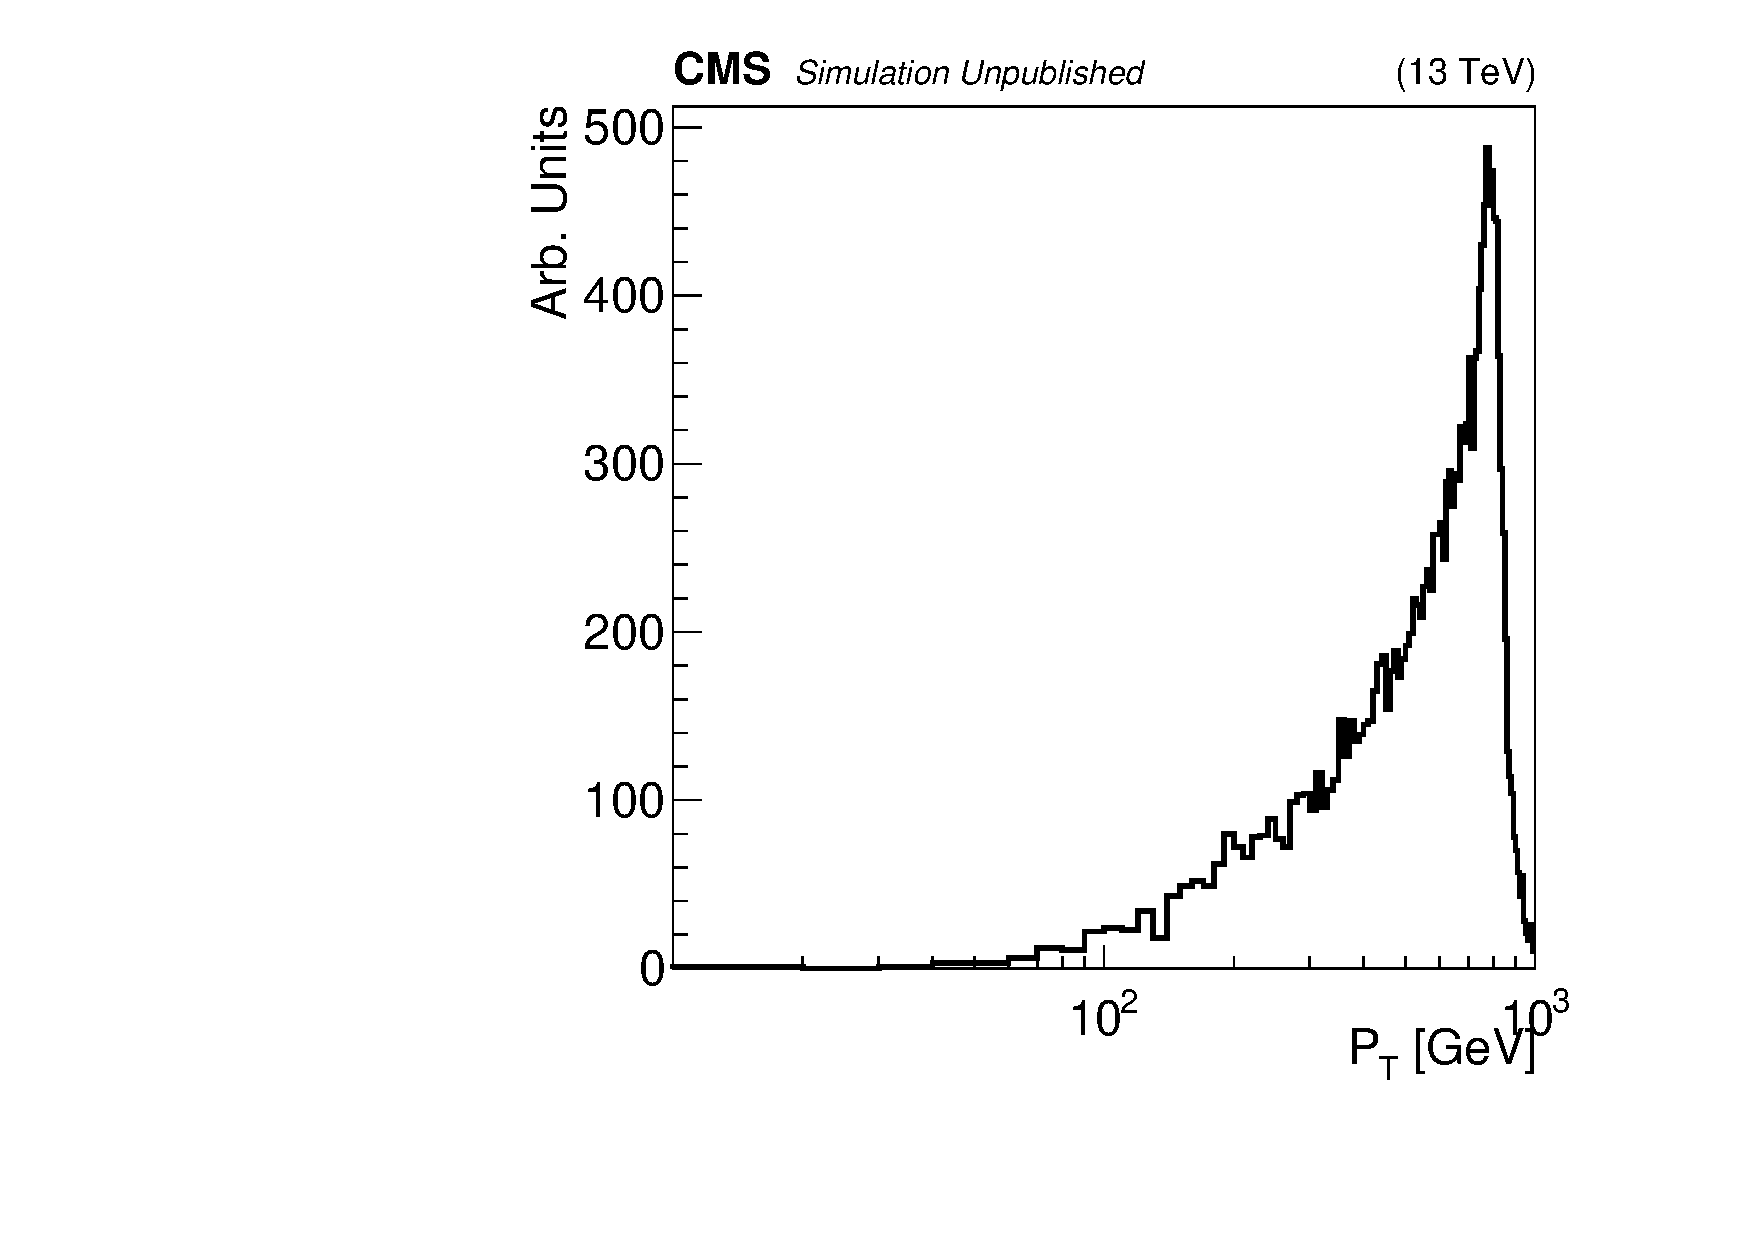
\includegraphics[width=2.4in]{figures/ptMatchedRecoEleFromWr_mwr2200_mnu1100.pdf}
		\caption{e from $\WR \rightarrow eN_{e}$}\label{fig:wrLeptJetPtsa}
	\end{subfigure}
	\thickspace
	\begin{subfigure}[t]{2.4in}
		\centering
		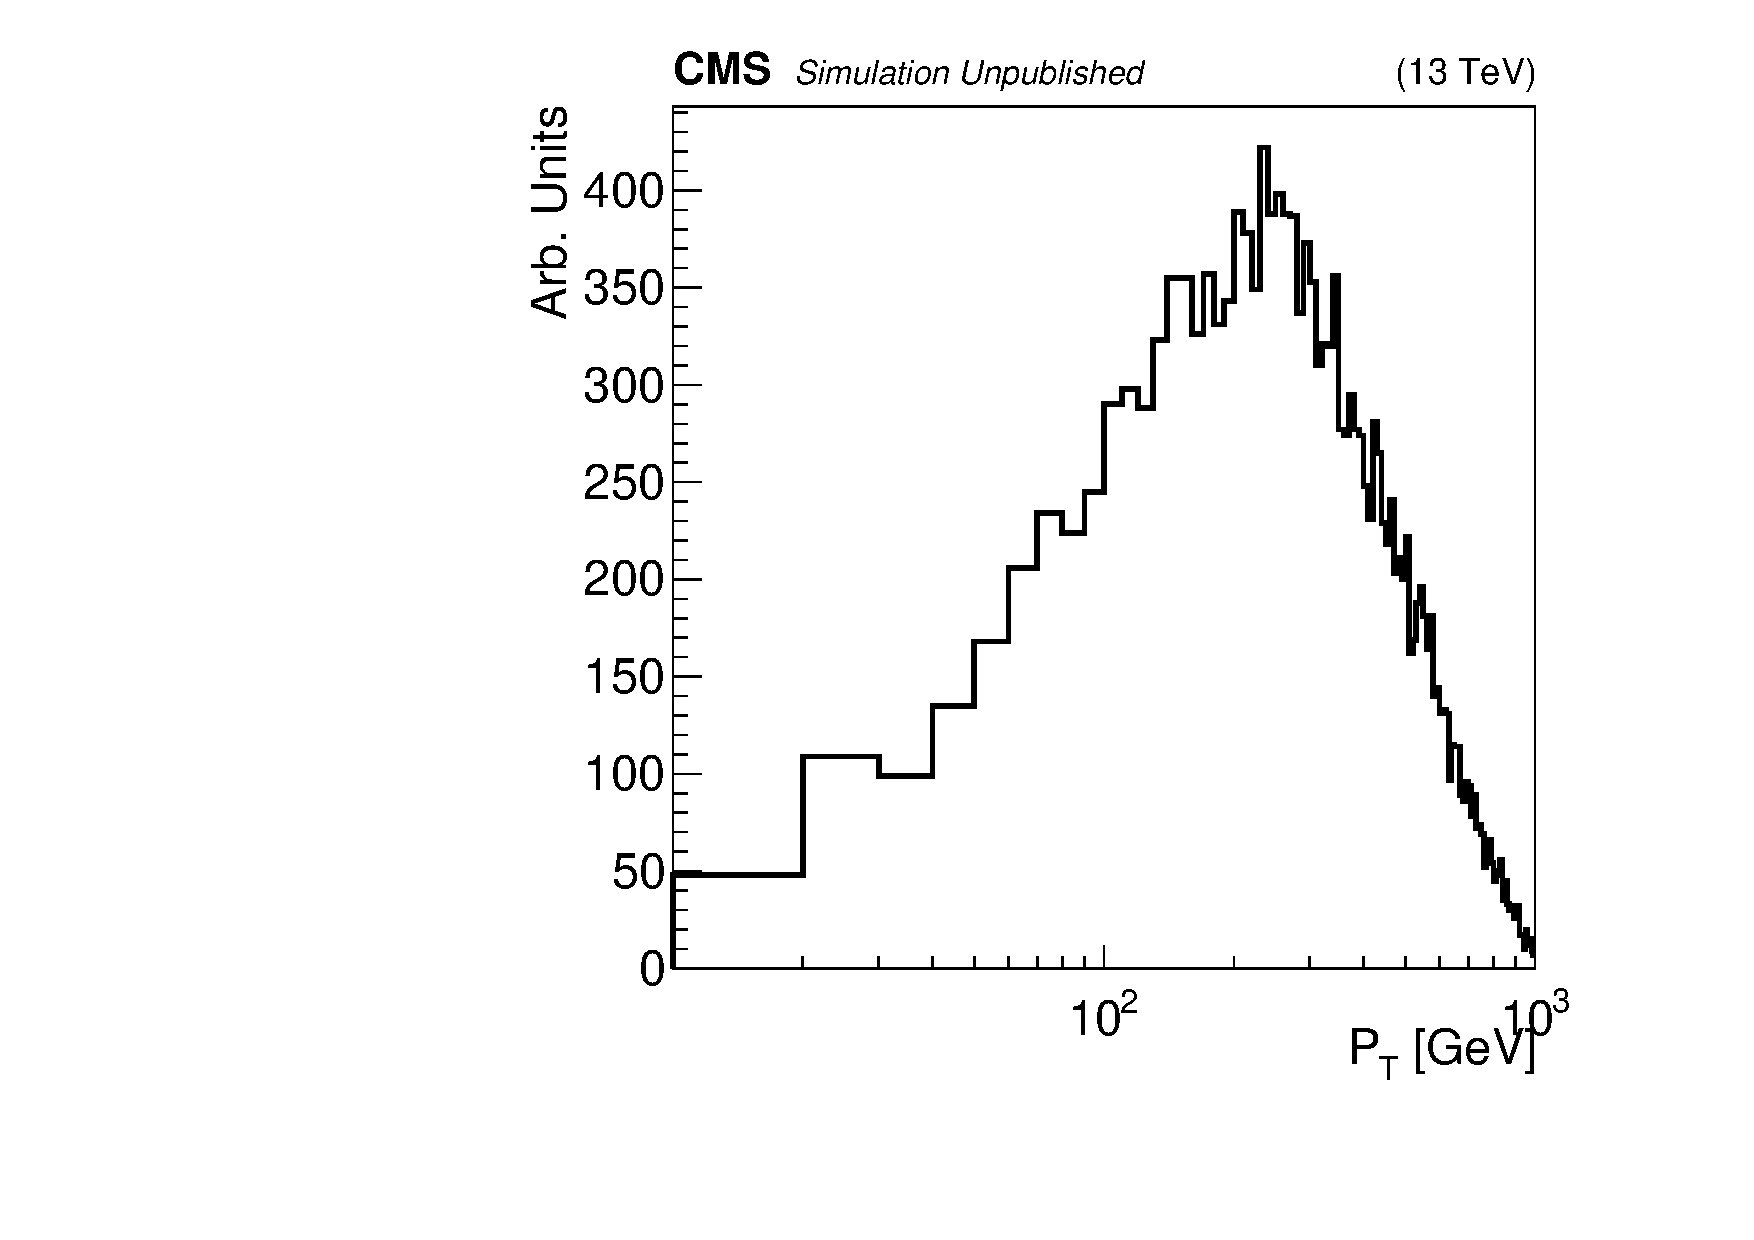
\includegraphics[width=2.4in]{figures/ptMatchedRecoEleFromNu_mwr2200_mnu1100.pdf}
		\caption{e from $N_{e} \rightarrow ejj$}\label{fig:wrLeptJetPtsb}
	\end{subfigure}
	\newline
	\newline
	\newline
	\newline
	\begin{subfigure}[t]{2.4in}
		\centering
		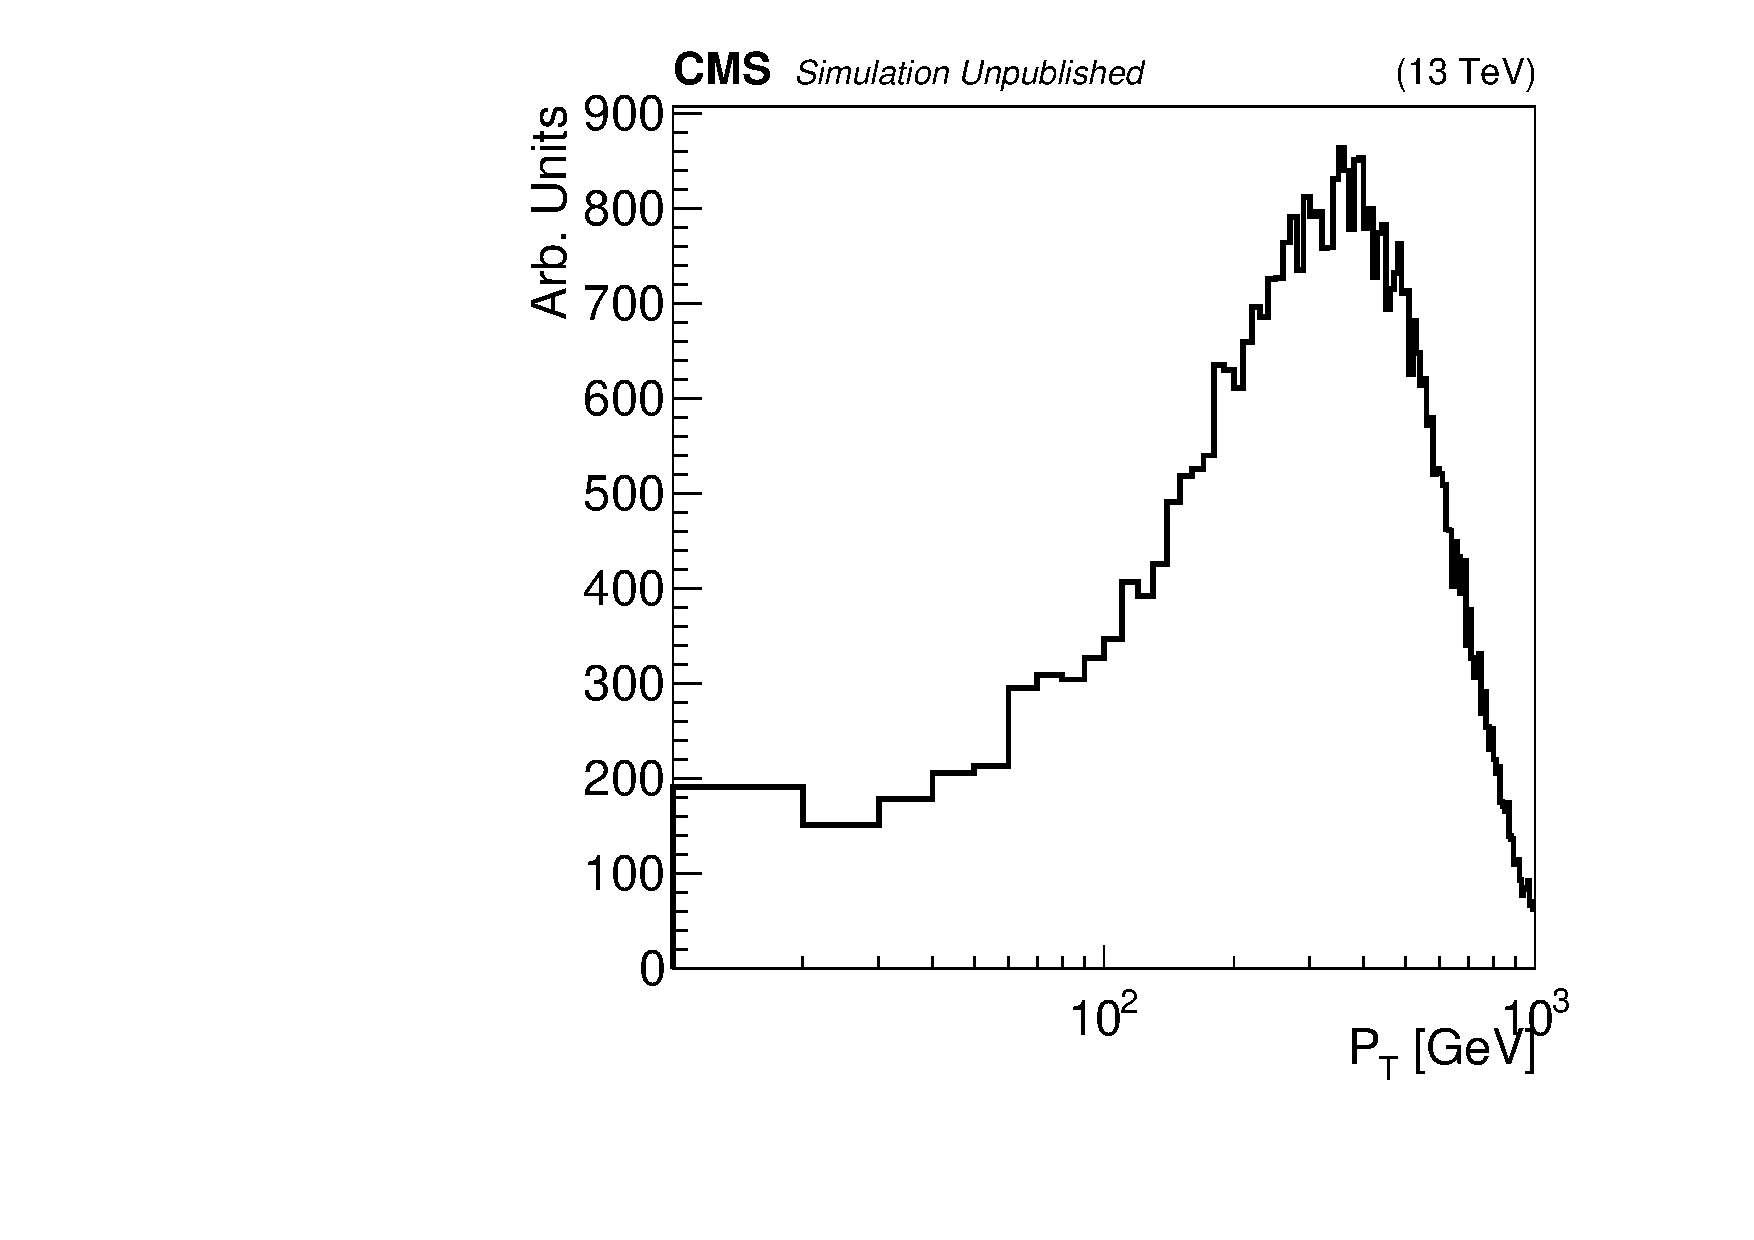
\includegraphics[width=2.4in]{figures/ptMatchedRecoJetOne_mwr2200_mnu1100.pdf}
		\caption{jet from $N_{e} \rightarrow ejj$}\label{fig:wrLeptJetPtsc}
	\end{subfigure}
	\thickspace
	\begin{subfigure}[t]{2.4in}
		\centering
		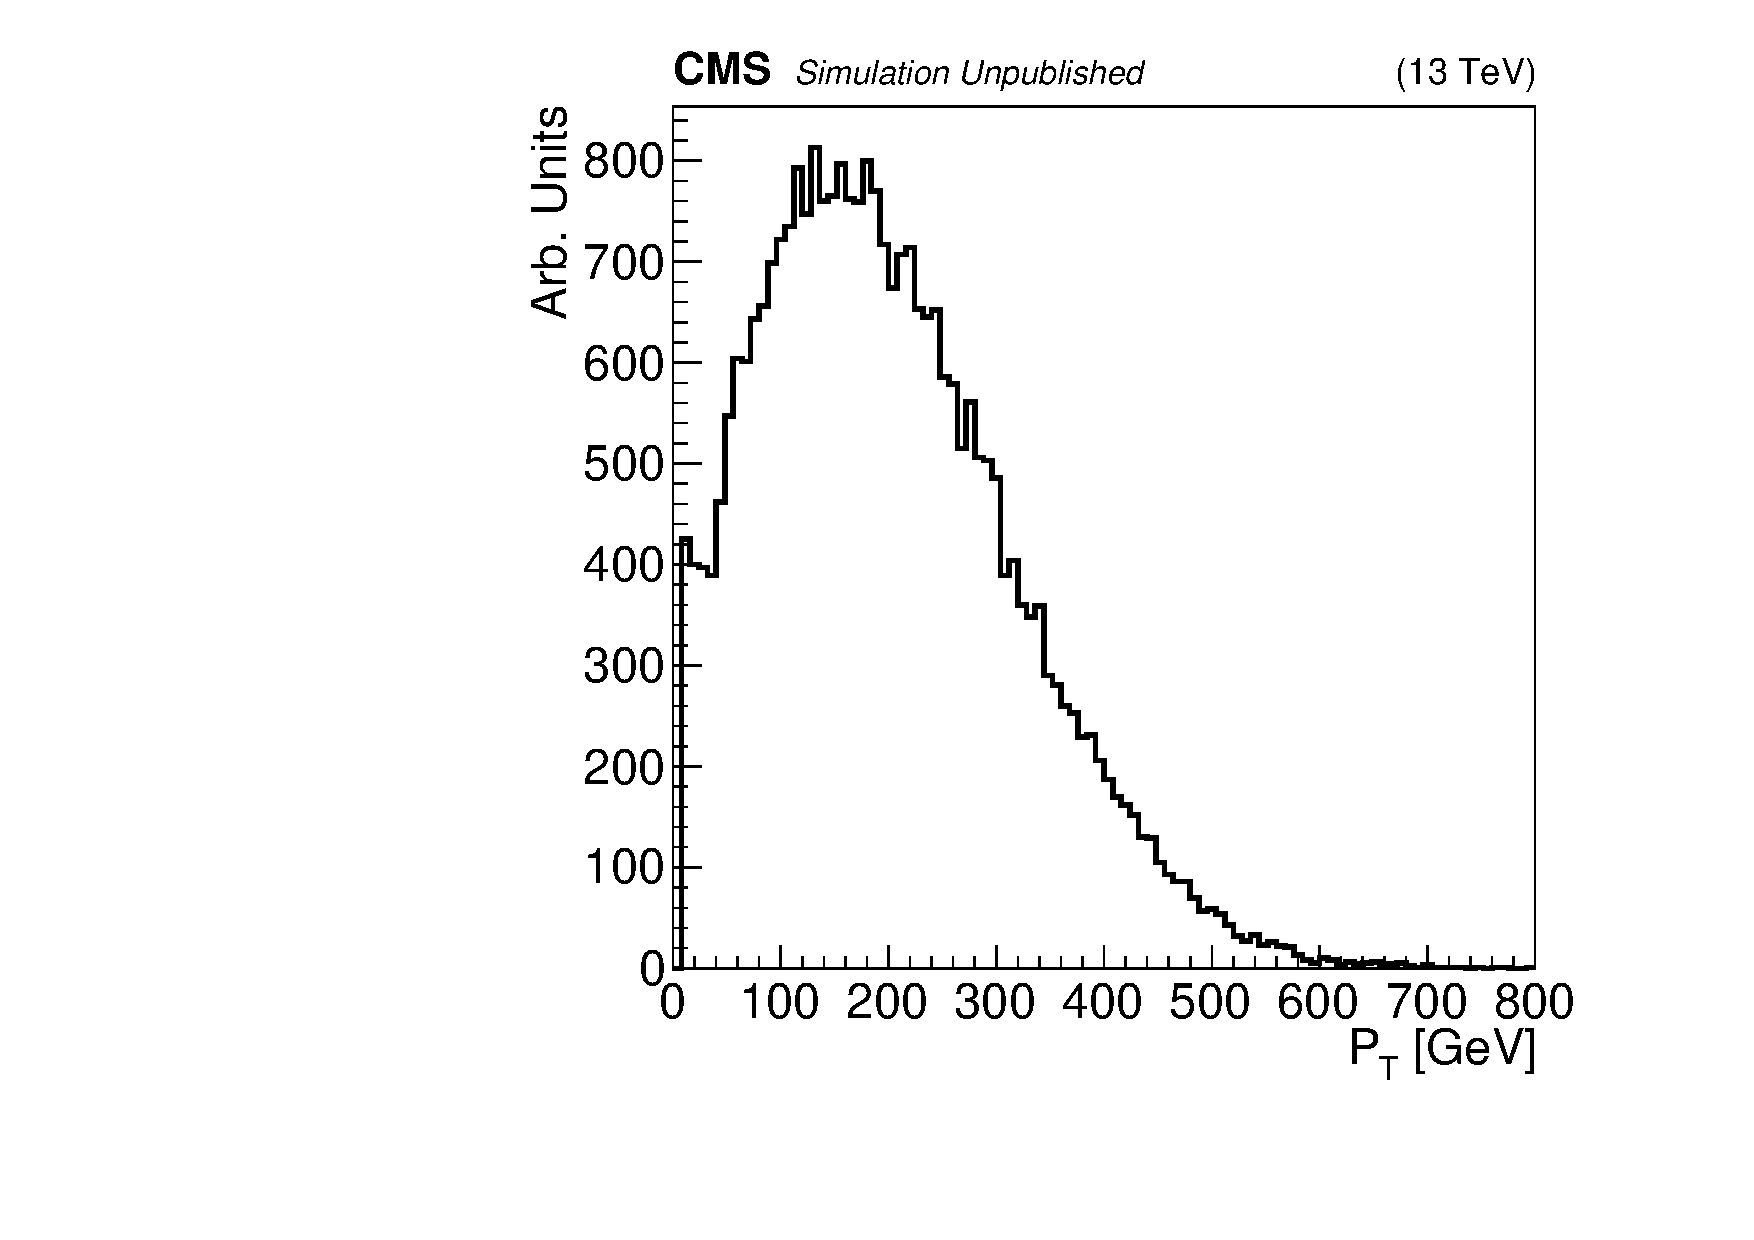
\includegraphics[width=2.4in]{figures/ptMatchedRecoJetTwo_mwr2200_mnu1100.pdf}
		\caption{jet from $N_{e} \rightarrow ejj$}\label{fig:wrLeptJetPtsd}
	\end{subfigure}
	\caption{The $\pt$ distributions of electrons and jets reconstructed in $\WR \rightarrow eejj$ events with $\mWR = 2.2$ $\TeV$ 
		and $\mnul = \frac{1}{2}\mWR$.}\label{fig:wrLeptJetPts}
\end{figure}

\begin{figure}
	\centering
	\begin{subfigure}[t]{2.4in}
		\centering
		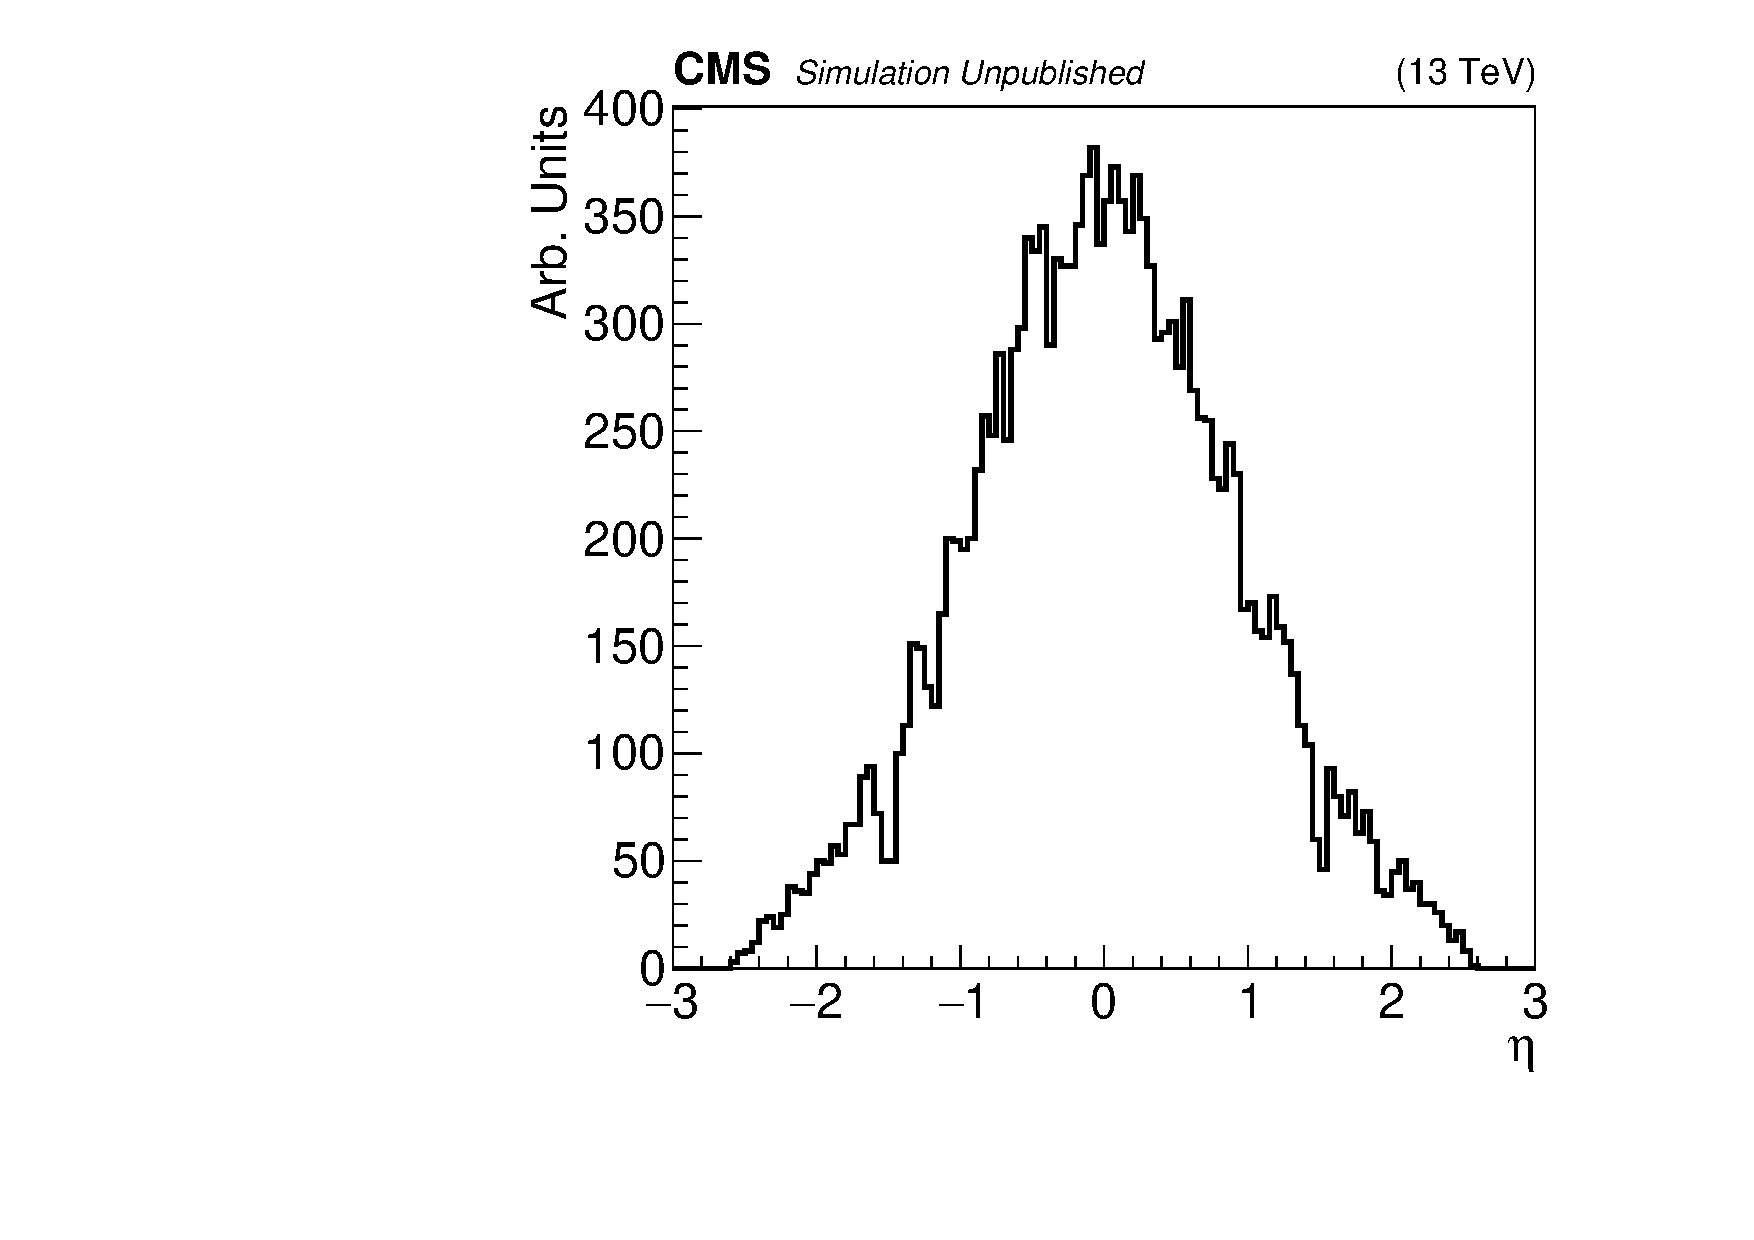
\includegraphics[width=2.4in]{figures/etaMatchedRecoEleFromWr_mwr2200_mnu1100.pdf}
		\caption{e from $\WR \rightarrow eN_{e}$}\label{fig:wrLeptJetEtasa}
	\end{subfigure}
	\thickspace
	\begin{subfigure}[t]{2.4in}
		\centering
		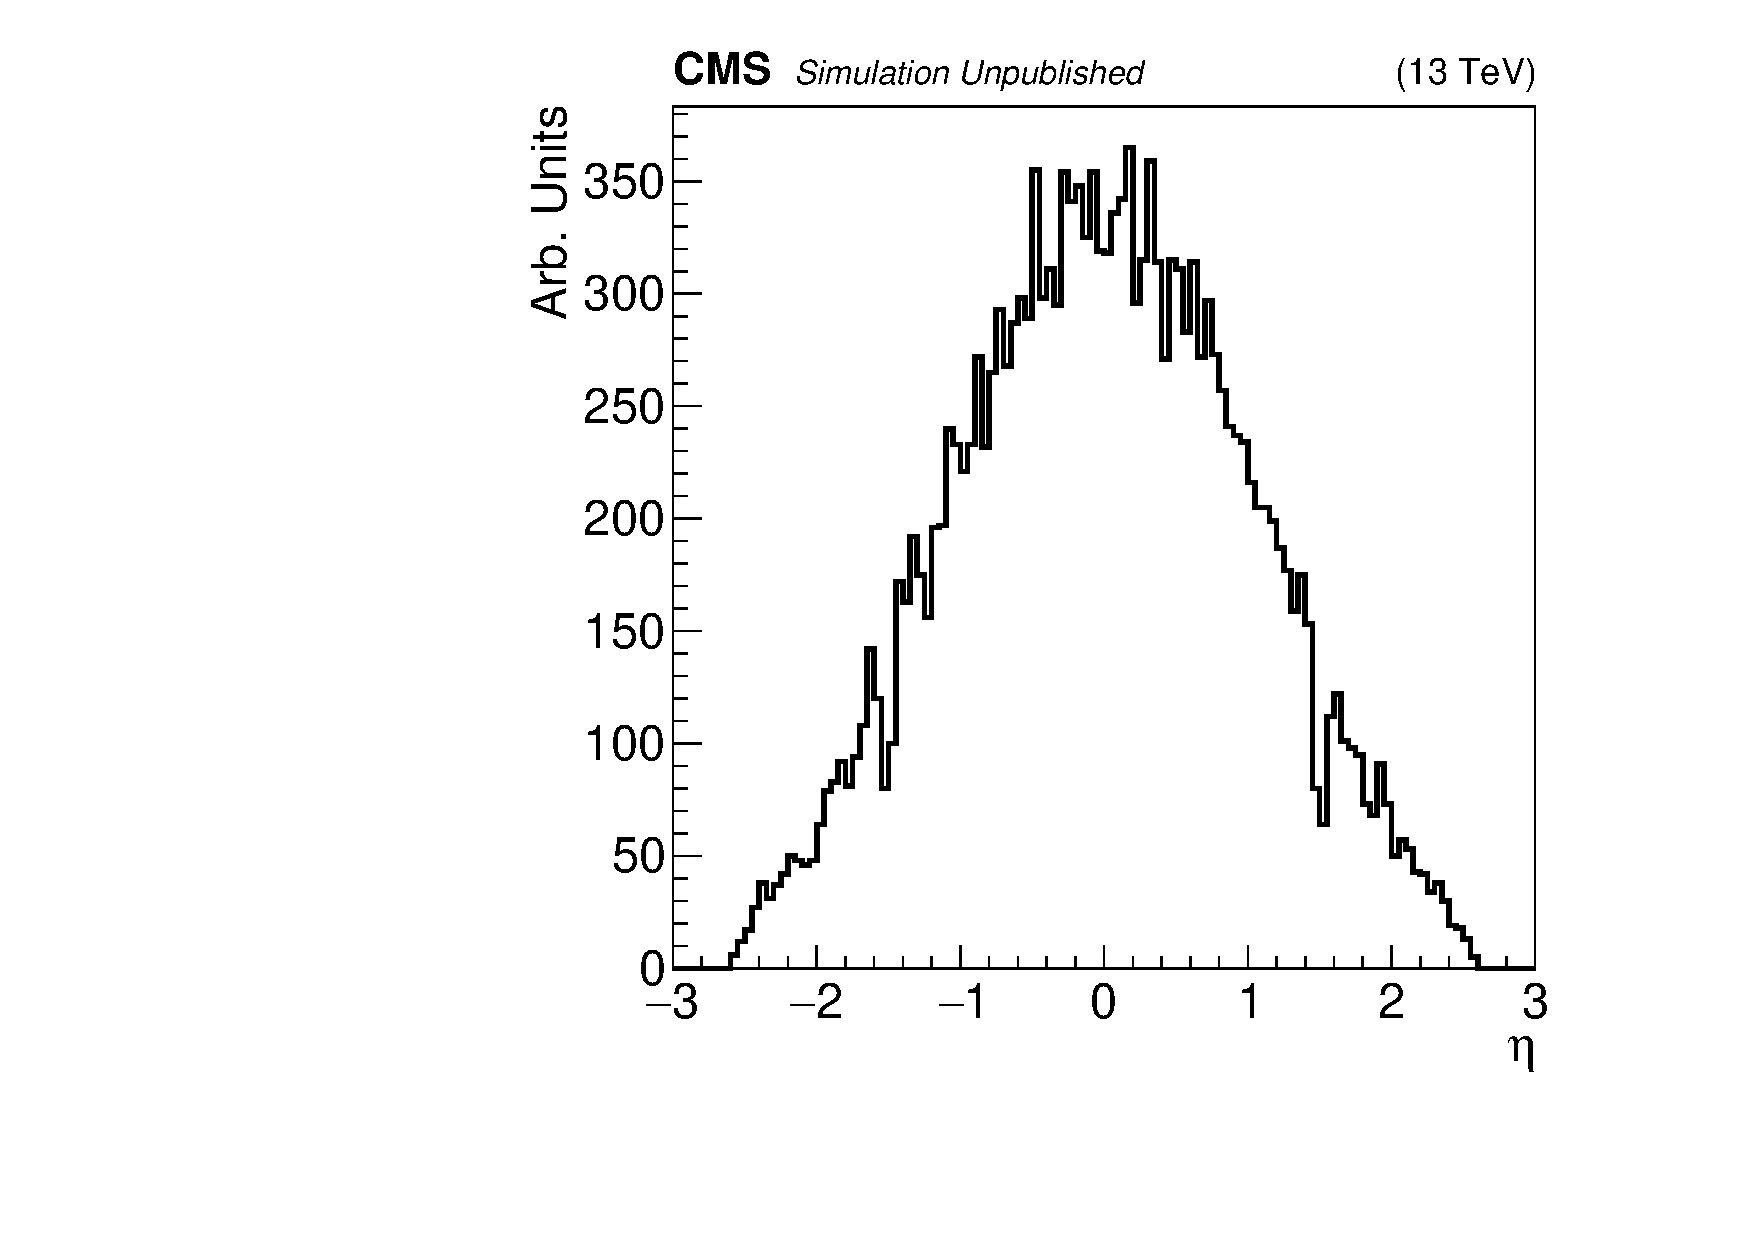
\includegraphics[width=2.4in]{figures/etaMatchedRecoEleFromNu_mwr2200_mnu1100.pdf}
		\caption{e from $N_{e} \rightarrow ejj$}\label{fig:wrLeptJetEtasb}
	\end{subfigure}
	\newline
	\newline
	\newline
	\newline
	\begin{subfigure}[t]{2.4in}
		\centering
		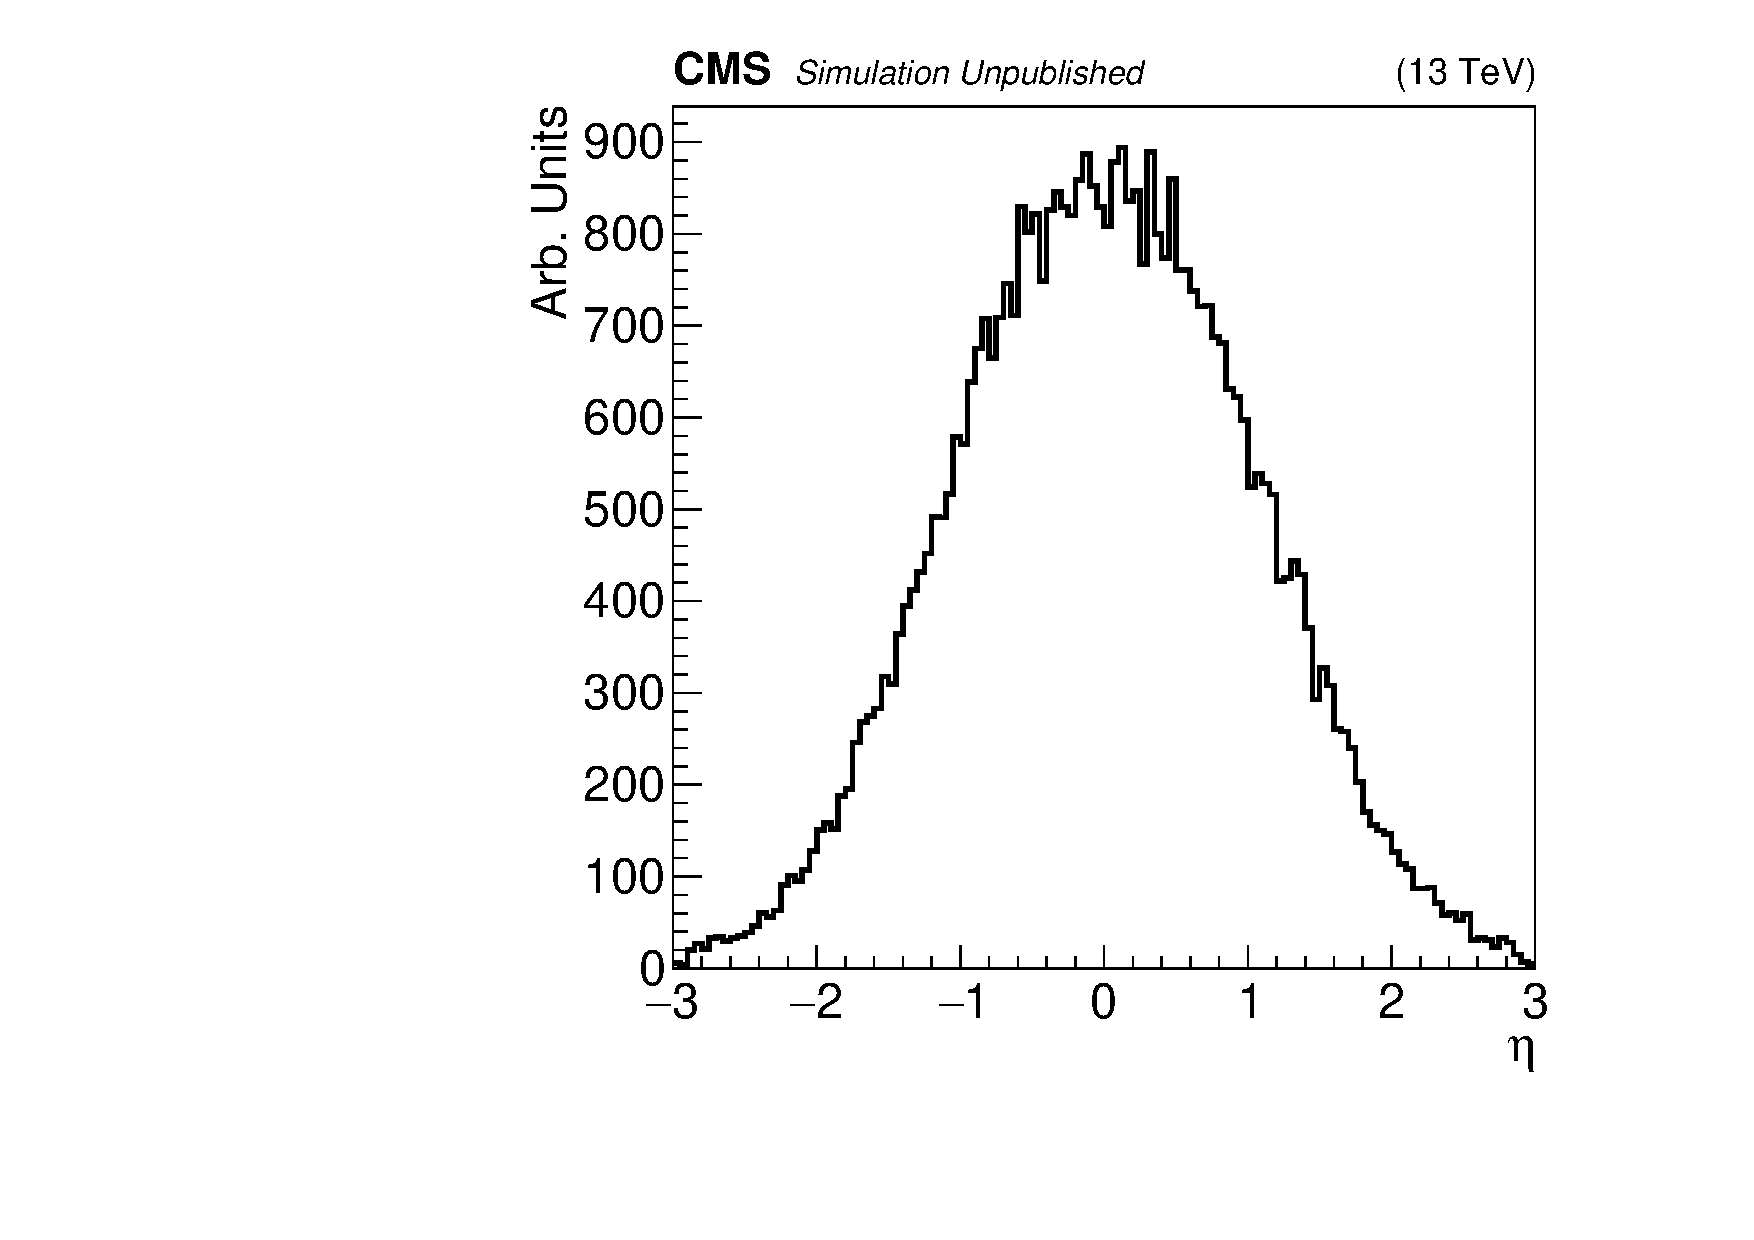
\includegraphics[width=2.4in]{figures/etaMatchedRecoJetOne_mwr2200_mnu1100.pdf}
		\caption{jet from $N_{e} \rightarrow ejj$}\label{fig:wrLeptJetEtasc}
	\end{subfigure}
	\thickspace
	\begin{subfigure}[t]{2.4in}
		\centering
		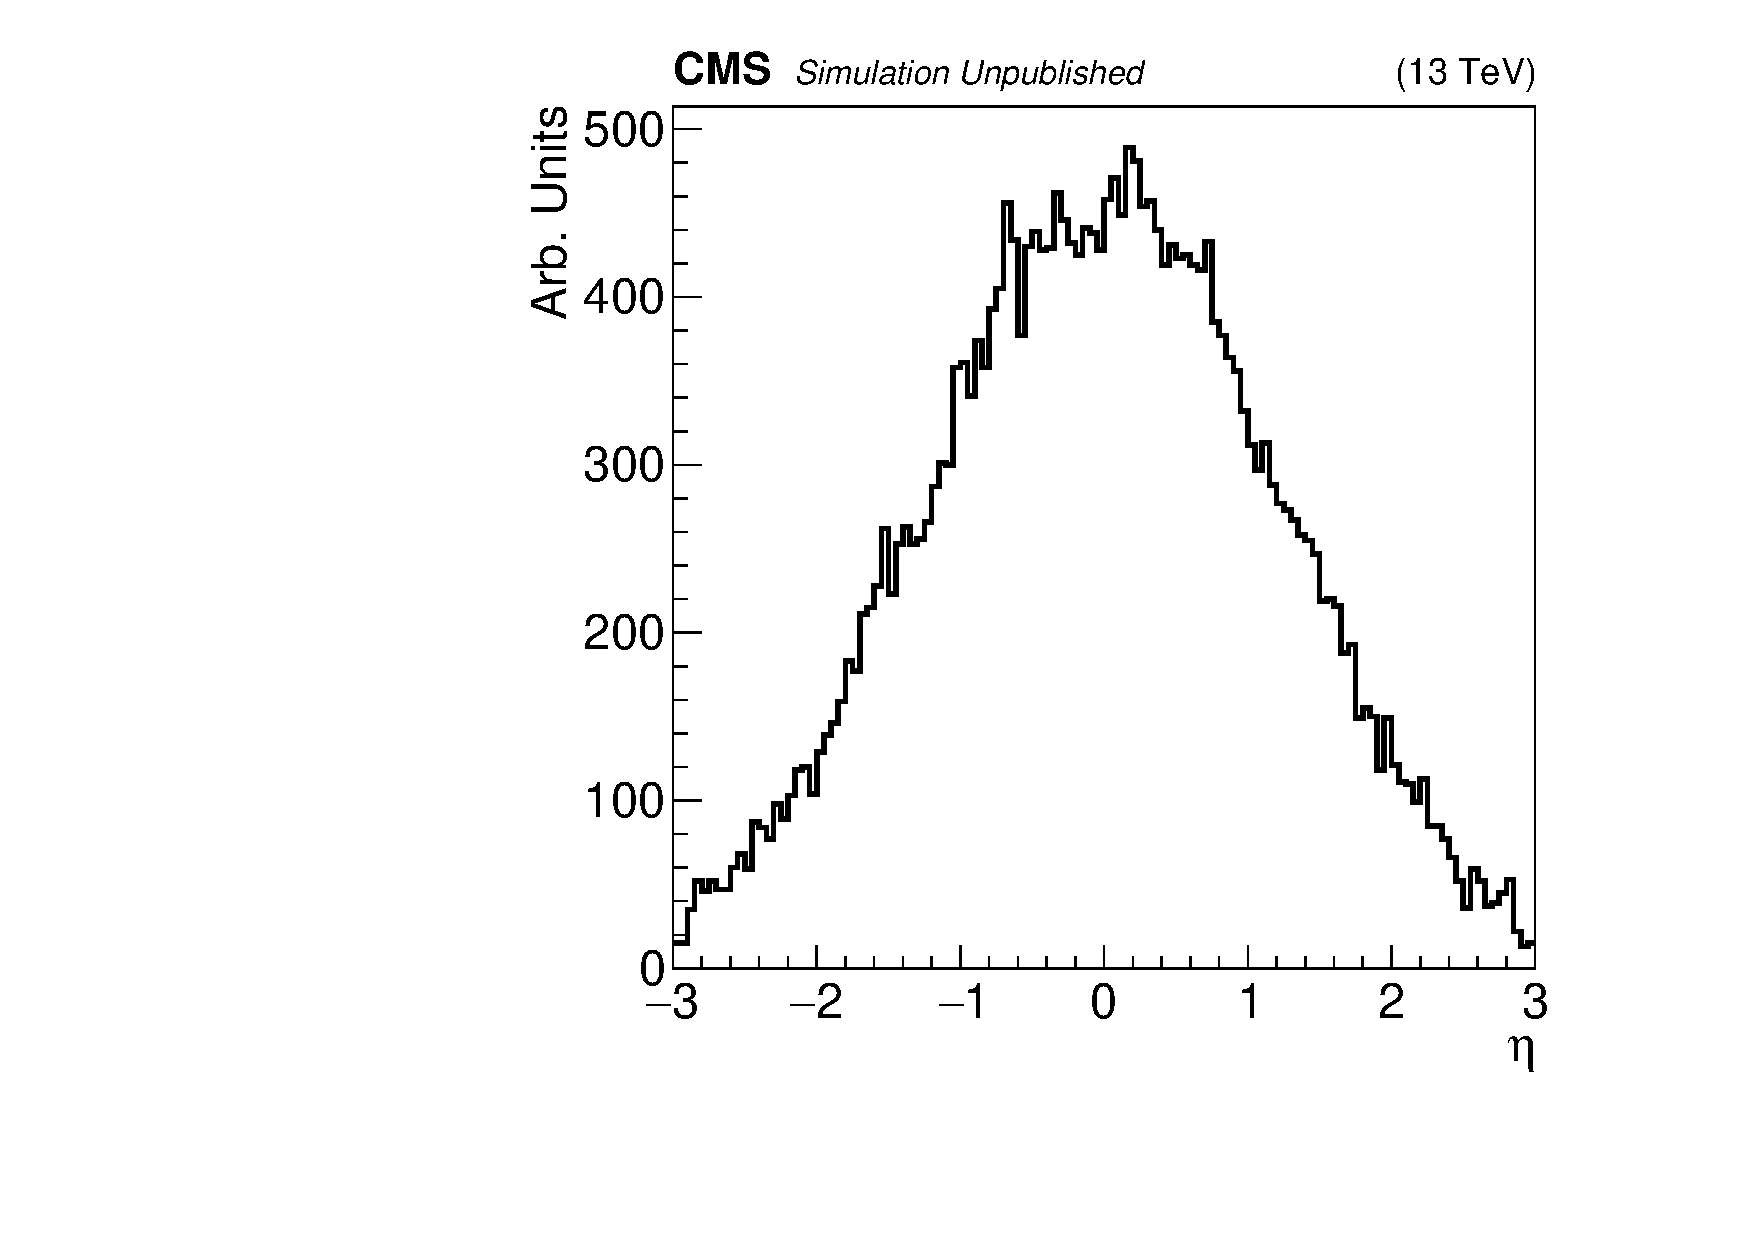
\includegraphics[width=2.4in]{figures/etaMatchedRecoJetTwo_mwr2200_mnu1100.pdf}
		\caption{jet from $N_{e} \rightarrow ejj$}\label{fig:wrLeptJetEtasd}
	\end{subfigure}
	\caption{The $\eta$ distributions of electrons and jets reconstructed in $\WR \rightarrow eejj$ events with $\mWR = 2.2$ $\TeV$ 
		and $\mnul = \frac{1}{2}\mWR$.}\label{fig:wrLeptJetEtas}
\end{figure}


%The event selections were driven by model independent features of \WR and \nul decays, and ST backgrounds in the $\ell\ell jj$ 
%final states.  The expected \WR mass (\mWR) is large, above 2 $\TeV$, relative to the 13 $\TeV$ collision energy, 
%so \WR bosons are expected to have low net momentum.  Therefore, the charged lepton and jet decay products, on average, 
%are distributed uniformly in $\phi$, and are concentrated in the $|\eta| < 2.4$ region\footnote{The $|\eta| < 2.4$ region 
%covers 94\% of the $0 \leq \theta < 180$ degree phase space, where $\theta = 0$ points along the beam axis.}, 
%as shown in Figures \ref{fig:wrLeptonEtas} and \ref{fig:wrJetEtas}.  Furthermore, the large expected \mWR means final 
%state leptons and jets should have $\pt$ of several hundred $\GeV$ or more, as shown in Figures \ref{fig:wrLeptonPts} and 
%\ref{fig:wrJetPts}.  In contrast, the ST backgrounds in the $\ell\ell jj$ final states produce leptons and jets primarily 
%with $\pt < 100$ $\GeV$, as shown in Figures \ref{fig:bkgLeptonPts} and \ref{fig:bkgJetPts}.  These differences in 
%lepton and jet kinematics between signal and background events motivated the following event selections:
%
%\begin{itemize}
%	\item Two leptons were reconstructed with $\pt > 53$ $\GeV$, and one with $\pt > 60$ $\GeV$.
%	\item Two jets were reconstructed with $\pt > 40$ $\GeV$.
%	\item Both leptons and jets were reconstructed with $|\eta| < 2.4$.
%	\item The invariant mass $\Mlljj$ of the reconstructed leptons and jets was greater than 600 $\GeV$.
%\end{itemize}
%
%The decay $\WR \rightarrow \ell_{1}\nul$ produces a charged lepton $\ell_{1}$ that is very light relative 
%to the \WR, so in the CM frame of the \WR, $\ell_{1}$ is equally likely to be emitted in any direction.  Subsequently, the decay 
%$\nul \rightarrow \ell_{2}\WR^{*} \rightarrow \ell_{2}jj$ produces a dijet system and a second charged lepton $\ell_{2}$.  As 
%long as $\mnul \gtrsim \mWR / 10$, the mass difference $\mnul - m_{\ell}$ produces a low velocity dijet system, and a high 
%velocity lepton $\ell_{2}$ that, on average, is separated from both jets by $\Delta R > 0.4$.  In the CM frame of the \nul, the 
%lepton $\ell_{2}$ is equally likely to be emitted in any direction.  Therefore, in $\sim$50\% of \WR decays the angular separation 
%between $\ell_{1}$ and $\ell_{2}$ measured in a plane that contains both of their momentum vectors is greater than $\frac{\pi}{2}$.  
%This separation causes the dilepton mass $\Mll$ to exceed $\sqrt{2} p_{1}p_{2}$, where $p_{i}$ is the momentum magnitude of 
%$\ell_{i}$.  Both leptons and jets are very light relative to the \WR, so on average the sum of lepton momentum magnitudes is 
%$p_{1} + p_{2} = \mWR / 2$, and their geometric mean is $p_{1}p_{2} = \mWR /\sqrt{8}$.  Thus, in $\sim$50\% of \WR decays the 
%difference between \mnul and $m_{\ell}$ results in a dilepton mass $\Mll > \mWR/2$.  In contrast, the two dominant backgrounds 
%- \DY and top quark processes - produce more than 50\% of their $\ell\ell jj$ events with $\Mll < 200$ $\GeV$, several hundred 
%$\GeV$ below $\mWR / 2$ for the majority of signal mass hypotheses tested in the search presented in this thesis.  In addition, 
%in QCD multijet and W+jets background events where two leptons were reconstructed, at least one lepton was often a byproduct of 
%hadronization, and was reconstructed near but not clustered into a jet.  These differences in the $\Mll$ and $\Delta R(\ell,j)$ 
%separation variables between signal and ST background events motivated the following event selections:
%
%\begin{itemize}
%	\item Each reconstructed lepton was separated from the other lepton and both jets by $\Delta R > 0.4$.
%	\item The dilepton mass $\Mll$ of the two reconstructed leptons was greater than 200 $\GeV$.
%\end{itemize}


\subsection{Kinematic Selection Criteria}


\section{Conclusion}
\label{sec:recoConclusion}
%conclusion for original reconstruction chapter, which did not include selection criteria
%Energetic electrons, muons and jets produced in collisions are reconstructed from signals measured in CMS sub-detectors and using 
%specialized reconstruction algorithms.  Reconstructed leptons and jets were required to pass additional selections to increase 
%sensitivity to a \WR signal relative to ST backgrounds.



%%%%%%%%%%%%%%%%%%%%%%%%%%%%%%%%%%%%%%%%%%%%%%%%%%%%%%%%%%%%%%%%%%%%%%%%%%%%%%%%
